%% vim: set sts=4 et tw=100 :

\chapter{Library Interface}
\label{ch:interface}

We begin this chapter by explaining the rationale behind several of the design decisions of the
EOS libraries in \refsec{interface:design}. Subsequently, we document the core set of C++ classes
in \refsec{interface:classes}.


\section{Design}
\label{sec:interface:design}

In order to fulfill its intended use cases, the EOS libraries are designed with concepts in mind.\\

First, most of the scalar quantities that used within the EOS libraries are treated as parameters.
These start with directy experimental input, such as particle masses and lifetimes. They continue
along the lines of more theoretically motivated quantities, such as quark masses (in the \MSbar{}
scheme) and the Wolfenstein parameters of the CKM matrix. It is therefore straightforward to change
a parameter's role within the scope of a theoretical analysis, from being a nuisance parameter in
the course of producing some estimates to being a genuine parameter of interest in the course of a
fit. In order to differentiate between the various parameters, a naming scheme is put in place.
Within this scheme, a parameter's name is rendered:
\begin{equation}
    \texttt{NAMESPACE::ID@TAG}\,,
\end{equation}
where the meta variables take the following meaning:
\begin{description}
    \item[NAMESPACE] A short description of the context in which the parameter should be
        interpreted. Possible namespaces include, but are not limited to: \texttt{mass},
        \texttt{decay-constants}, \texttt{CKM}, and others. \\
    \item[ID] A handle for a parameter in a given namespace.\\
    \item[TAG] Usually a reference, which allows to distinguish between parameters with the same
        \texttt{ID}.\\
\end{description}

Second, if a quantity exhibits a functional dependence on either a parameter or
a kinematic variable, it is treated in a modular fashion. Per default, an
abstract interface is created that allows for several implementation of the
same quantity. The actual implementations of this interface are then accesible
via a factory method. An excellent example for such a \emph{plugin} design is
found within the scope of hadronic matrix elements, in particular hadronic form
factors. Each implementation of a plugin usually depends on its own set of
parameters. For clarity, we use one of the hadronic form factor as an example.
Consider the $B\to \pi$ vector form factor $f^{B\pi}_+$. One possible
parametrization of this form factor has been proposed in \cite{Bourrely:2008za}
(BCL2008). It is achieved in terms of three parameters: the normalization
$f^{B\pi}_+(0)$, and two shape parameters $b^{B\pi,+}_1$ and $b^{B\pi,+}_2$.
This parametrization is implemented within EOS, andobservables that depend on
the $B\to \pi$ form factors can choose it through the option
\texttt{form-factors=BCL2008}. The relevant parameters are contained in the
namespace \texttt{B->pi}, and tagged for the \text{BCL2008} plugin:
\begin{equation}
    \texttt{B->pi::f\_+(0)\@BCL2008}\,,\quad\texttt{B->pi::b\_+\^{}1\@BCL2008}\,,
    \quad\text{and}\quad\texttt{B->pi::b\_+\^{}2\@BCL2008}\,.
\end{equation}
As such, there is no risk of namespace collisions among the various plugins'
parameters.\\


Third, \dots

{Likelihood and Prior}
\begin{itemize}
    \item construct likelihood and prior at run time
    \item abstract tree, with leaves:
    \begin{itemize}
        \item (Multivariate) Gaussian distribution
        \item LogGamma distribution (for asymmetric uncertainty intervals)
        \item Amoroso (for limits)
        \item Flat (prior only)
    \end{itemize}
\end{itemize}


\section{Core Classes}
\label{sec:interface:classes}

At the core of the EOS API there are four classes -- \class{Parameters}, \class{Kinematics},
\class{Options}, \class{Observable} -- all of which are discussed in the following.

\subsection{Class \class{Parameters}}

\texttt{key = value} dictionary, with string keys and floating-point real values\\

\begin{itemize}
    \item copies share, by default, the parameters of the original
    \item observables usually share a common set of parameters
\end{itemize}

\begin{figure}[t]
    \centering
    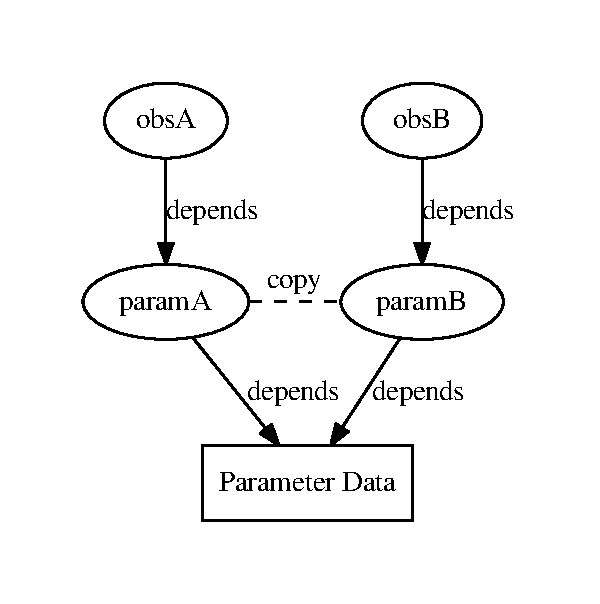
\includegraphics[width=.5\textwidth]{figures/graph-parameters.pdf}
    \caption{%
        Diagrammatic illustration that multiple observables can depend on the
        very same instance of \cpp{Parameters}.
    }
\end{figure}

\begin{sourcecode}
Parameters paramA = Parameters::Defaults();
Parameters paramB(paramA);

ObservablePtr obsA = Observable::make("A", paramA, Kinematics{ }, Options{ });
ObservablePtr obsB = Observable::make("A", paramB, Kinematics{ }, Options{ });
\end{sourcecode}

\begin{itemize}
    \item access to individual parameters via array subscript \texttt{[\,]}
    \begin{itemize}
        \item input: parameter name
        \item result: instance of \class{Parameter},
            w/ persistent access to parameter data\\
            {lookup once, use often!}
    \end{itemize}
    \item parameter naming scheme: \texttt{NAMESPACE::ID@SOURCE}, e.g.:\\
    \begin{itemize}
        \item \texttt{mass::b(MSbar)} $\to$ mass $\overline{m}_b(\overline{m}_b)$ in \MSbar{} scheme
        \item \texttt{B->K::f\_+(0)@KMPW2010} $\to$ normalization of $f_+$ FF in $B\to K$ decays, according to KMPW2010
    \end{itemize}
\end{itemize}

\subsection{Class \class{Kinematics}}

The class \class{Kinematics} is a dictionary from \cpp{std::string}-valued keys to
\cpp{double}-valued entries. Upon construction of an observable, a suitable instance
of kinematics is bound to that observable.

\texttt{key = value} dictionary, with string keys and floating-point real values

\begin{itemize}
    \item allows run-time construction of observables
    \item each obervable has its very own set of kinematic variables
    \item access to individual variables via array subscript {\texttt{[\,]}}
    \begin{itemize}
        \item input: variable name
        \item result: double
    \end{itemize}
    \item no naming scheme, since namespace is unique per observable instance
\end{itemize}

\subsection{Class \class{Options}}

\texttt{key = value} dictionary, with string keys and string values
influences how observables are evaluated

\begin{itemize}
    \item access to individual otions via array subscript {\texttt{[\,]}}
    \begin{itemize}
        \item input: option name
        \item result: string value
    \end{itemize}
    \item example: lepton flavour in semileptonic decay:\\
        \texttt{l=mu}, \texttt{l=tau}, \dots
    \item example: choice of form factors:\\
        \texttt{form-factors=KMPW2010}\, \dots
    \item example: \texttt{model=\dots} as choice of underlying physics model
    \begin{description}
        \item[\texttt{SM}] to produce SM prediction
        \item[\texttt{WilsonScan}] to fit Wilson coefficients
        \item[\texttt{CKMScan}] to fit CKM matrix elements
    \end{description}
\end{itemize}

\subsection{Class \class{Observable}}

\class{Observable} is an abstract base class\\

\begin{itemize}
    \item Its descendants must at construction time:
        \begin{itemize}
            \item associate with an instance of Parameters
            \item extract values from their instance of Options
        \end{itemize}

    \item Their construction occurs via factory method, e.g.:\\
       \cpp{Observable::make("B->pilnu::BR", p, k, o)}

       The latter creates an observable at runtime using the observable's name (here:
       \texttt{B->pilnu::BR}), a set of parameters \cpp{p}, a set of kinematic variables \cpp{k},
       and a set of options \cpp{o}.

    \item Any changes to the observable's instance \cpp{p} of \class{Parameters} after construction
       of the observable transparently affect the observable, and all further observable associated with \cpp{p}.

    \item Any changes to \cpp{o} of \class{Options} do not affect the observable after construction time.

    \item Observables can be
        \begin{itemize}
            \item evaluated via \cpp{evaluate}:\\[\smallskipamount]
              This methods runs the necessary computations for the present values of the parameters\\[\smallskipamount]

            \item copied:\\[\smallskipamount]
              The copy-constructor does not create an independent copy; the new object rather uses the same
              parameters, with the same options as the original.\\[\smallskipamount]

            \item cloned:\\[\smallskipamount]
              The method \cpp{clone} creates an independent copy of the same observable, using a different set of
              parameters than the original
        \end{itemize}

    \item All users of \class{Observable} must also support cloning. This allows to easily parallelize algorithms
        within EOS.
\end{itemize}

\begin{figure}
    \subfigure[copy]{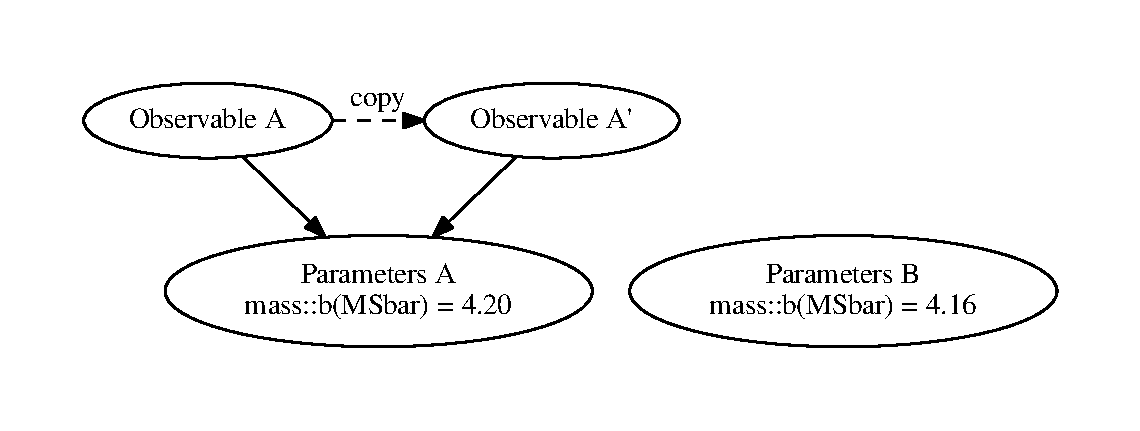
\includegraphics[width=.5\textwidth]{figures/graph-observable-copy.pdf}}
    \subfigure[clone]{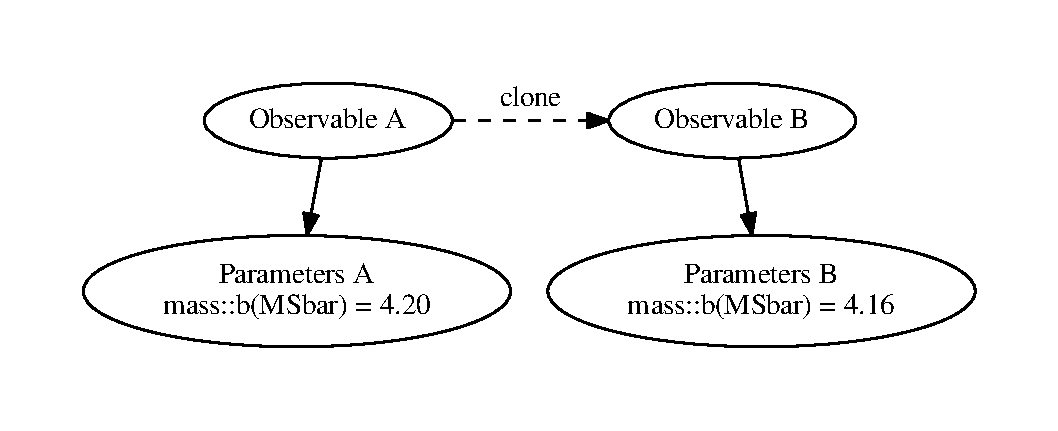
\includegraphics[width=.5\textwidth]{figures/graph-observable-clone.pdf}}
    \caption{%
        Diagrammatic illustration of the differences between copying an instance of
        \cpp{Observable} via the copy-constructor, and cloning the observable via the \cpp{clone}
        method
    }
\end{figure}
